\chapter{Elliptical photon distribution}
\label{EllipticalPhotonDistribution}

In order to compute where in the elliptical footprint a photon hits, one needs to create a function that translates a random number to an offset in the semimajor axis (since the height difference is independent of the semiminor axis location). This function can be computed using the inverse function of the integral function of the ellipse function (normalized by area). This transformation is based in the equation of the ellipse.

\begin{equation}
	\frac{x^2}{a^2}+\frac{y^2}{b^2}=0
\end{equation}

From this, the normalized y coordinate can be extracted and the integral can be defined. The function that then maps a coordinate on the a-axis to its probability is given in equation \ref{eq:yComp}.


\begin{equation}
	f(x) = \left. \left(2 \sqrt{b^2-\frac{b^2 x^2}{a^2}}\right)\right/(a b \pi);
	\label{eq:yComp}
\end{equation}
\begin{equation}
	h(x,a,b) = \int f(x) dx
\end{equation}
\begin{equation}
	i(x,a,b) = h(x,a,b)-\lim_{x_2\to-a} h(x_2,a,b)
	\label{eq:distributionCDF}
\end{equation}

Equation \ref{eq:distributionCDF} is too complex to solve analytically and is very computationally intensive for numerical approximation. To that purpose, an approximation is used in the form of a normal function with zero variance and a mean based on the semi-major axis. In figure \ref{fig:CDFcomparison}, a comparison is given between the approximation (purple) and the real function (blue). The final function can now be found by inverting equation \ref{eq:approxCDF}. The result can then be simplified to equation \ref{eq:EllipticalAreaInvCDF} which maps a random number between zero and one to the offset on the semimajor axis of the photon hit.

\begin{equation}
	y(x,a) = NormalCDF(0, 0.5a);
	\label{eq:approxCDF}
\end{equation}
\begin{equation}
	x = 0.707107 a \cdot InverseErf(2y-1)
	\label{eq:EllipticalAreaInvCDF}
\end{equation}

\begin{figure}[ht]
	\centering
	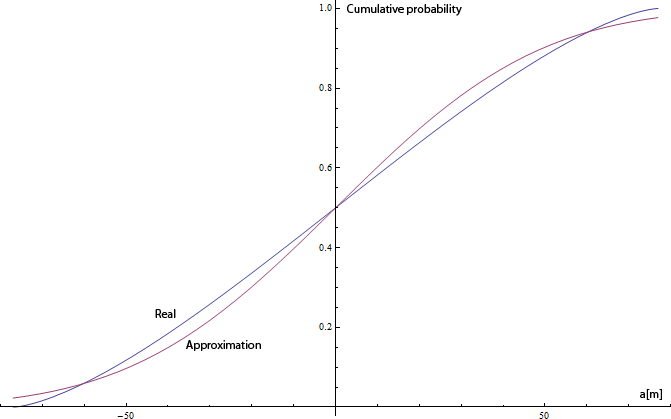
\includegraphics[width=1\textwidth, angle = 0]{chapters/img/ellipticalArea.png}%
		\caption{Cumulative probability on photon hit over the a-axis}%
		\label{fig:CDFcomparison}
\end{figure}